\section{Refinement}  \label{SEC_REFINEMENT}
The operation of \textit{refining} a cell is defined as dividing it
into eight equal cubic cells. When a cell is refined, the cell node
which represents it in the graph structure is replaced by a
structure consisting of eight cell nodes and six transition nodes,
which is similar to the initial graph. In order to exemplify the
refinement process, consider the refinement of cell number $0$ in
the mesh of Figure \ref{FIG_MESH_REFINEMENT}(a).

%FIG_MESH_REFINEMENT
\begin{figure}[!ht]
    \centering
    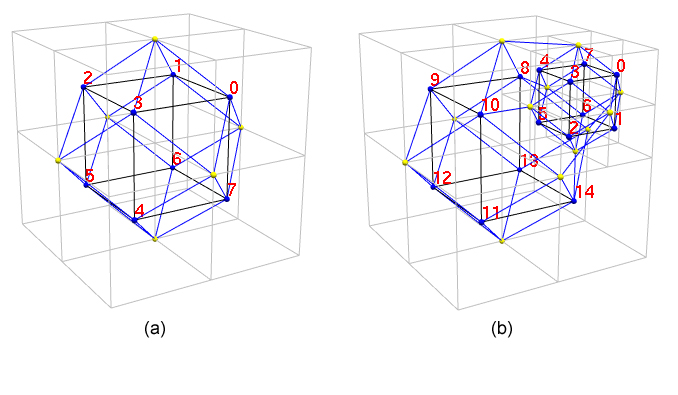
\includegraphics[scale=0.45,angle=0]{../img/gridAndGraph.jpg}
    \caption{Refinement of one cell.}
    \label{FIG_MESH_REFINEMENT}
\end{figure}

\noindent After refinement, cell $0$ will be divided into eight
smaller cells, half the length of the original one, with centers

\[
  \left(\frac{7}{8},\frac{7}{8},\frac{7}{8}\right),
  \left(\frac{7}{8},\frac{7}{8},\frac{5}{8}\right),
  \left(\frac{7}{8},\frac{5}{8},\frac{5}{8}\right),
  \left(\frac{7}{8},\frac{5}{8},\frac{7}{8}\right),
\]

\[
  \left(\frac{5}{8},\frac{7}{8},\frac{7}{8}\right),
  \left(\frac{5}{8},\frac{7}{8},\frac{5}{8}\right),
  \left(\frac{5}{8},\frac{5}{8},\frac{5}{8}\right),
  \left(\frac{5}{8},\frac{5}{8},\frac{7}{8}\right),
\]
resulting in the mesh of Figure \ref{FIG_MESH_REFINEMENT}(b).

More generally, when a cell centered at $(a, b, c)$ and length $L$
is refined, it is replaced by eight cells with length $L/2$ and
centers
\[
\left(a-\frac{L}{4},b-\frac{L}{4},c-\frac{L}{4}\right),
\left(a+\frac{L}{4},b-\frac{L}{4},c-\frac{L}{4}\right),
\left(a-\frac{L}{4},b+\frac{L}{4},c-\frac{L}{4}\right),
\]
\[
\left(a-\frac{L}{4},b-\frac{L}{4},c+\frac{L}{4}\right),
\left(a+\frac{L}{4},b+\frac{L}{4},c-\frac{L}{4}\right),
\left(a+\frac{L}{4},b-\frac{L}{4},c+\frac{L}{4}\right),
\]
\[
\left(a-\frac{L}{4},b+\frac{L}{4},c+\frac{L}{4}\right),
\left(a+\frac{L}{4},b+\frac{L}{4},c+\frac{L}{4}\right).
\]

The group of eight cells arising from a single original cell through
refinement will be called a \textit{bunch}. The cells of the new
bunch are ordered by the modified Hilbert curve, as will be
explained in Section \ref{SEC_HILBERT_CURVE}. The creation and
ordering of the new bunch of cells is merely a local event, which
alters only the states of the neighboring cells of the original
cell. These neighbor cells accordingly need to be notified of the
local change in the graph structure.

A cell that was just refined receives as its refinement level the level of the original unrefined cell plus one.
By convention, the cells of the initial mesh possess refinement
levels equal to $1$. In Figure \ref{FIG_MESH_REFINEMENT}(b), for
instance, cells number $0$ to $7$ have refinement level $2$, while
the remaining cells possess refinement level $1$. Transition nodes
are also assigned refinement levels, equal to the refinement levels
of the cells of the bunch in which they were created.

The length of a cubic cell $L$ relates to its refinement level $n$
through the simple relation

\begin{equation} \label{EQ_EDGE_SIZE}
 L = \frac{1}{2^n}.
\end{equation}

\subsection{Mesh refinement}
Mesh refinement is done according to criteria laid out by the
specific application. In the typical setting of adaptive mesh
refinement (AMR), when the variation of some physical variable in
the cells within a region of the computational domain exceeds some
preset value, called here the \textit{refinement bound}, indicating
that more precision might be needed in order to obtain more accurate
results, the program decides that the cells belonging to that region
must be refined. The program traverses the entire mesh in each
global iteration of the computations, verifying if any cell
satisfies the refinement condition defined by the application. When
a visited cell satisfies the condition, it is refined, originating a
modified mesh and its associated graph for the next global iteration
of the program.

Algorithm \ref{REFINEMENT_PROCEDURE} describes function
\textit{refine()}, which is responsible for the mesh refinement. It
receives as parameters the \textit{minimum refinement level} desired
for the mesh's cells, which is related to the minimum mesh size
initially expected necessary in order to get a reasonably meaningful
approximation to the solution of the problem being studied, and the
refinement bound discussed above.

\alglanguage{pseudocode}
\begin{algorithm}[!ht]
    \caption{Mesh refinement}
    \small{
    \begin{algorithmic}[1]
    \Procedure{refine}{minLevel, refinementBound}
        \State $CellNode \hspace{2mm} currentCell$
        \State $CellNode \hspace{2mm} auxiliar$
        \State $continueRefining \gets true$
        \While{$continueRefining$}
            \State $currentCell \gets firstCell$
            \State $continueRefining \gets false$
            \While{$currentCell$ is not $null$}
                \If{$currentCell.level < minLevel$ \textbf{and} the local spatial variation of some
                property in the cell exceeds the refinement bound}
                    \State $auxiliar \gets currentCell$
                    \State $currentCell \gets currentCell.next $
                    \State $refineCell(auxiliar)$
                    \State $numberOfCells \gets numberOfCells + 7$
                    \State $continueRefining \gets true$
                \Else
                    \State$currentCell \gets currentCell.next$
                \EndIf
            \EndWhile
        \EndWhile
    \EndProcedure
    \end{algorithmic}
    }
    \label{REFINEMENT_PROCEDURE}
\end{algorithm}

Notice in Algorithm \ref{REFINEMENT_PROCEDURE} that the attribute
that stores the number of cell nodes increases by $7$ at each cell
refinement and not by $8$. This happens because the cell node which
originated the new bunch is not stored as it would be in a typical
tree structure, but is completely replaced by the new bunch.
Moreover, in order to augment the performance, the cell node is not
actually destroyed upon refinement but is transformed into part of
the new bunch (specifically, it becomes the front northeast cell
node, as will be explained in the following). Thus, only $7$ new
cell nodes are created when a cell is refined.

\subsection{Cell refinement} \label{SUBSEC_PROCEDURE_REF}
The refinement of one cell is done by the function
\textit{refineCell()}. The process occurs in seven steps as
described below. Each step will be presented afterwards in a
detailed algorithm.

\begin{enumerate}
 \item Transformation of the cell to be refined into the front northeast cell of the new
 bunch.
 \item Creation of the remaining 7 cell nodes of the new bunch.
 \item Creation of 6 transition nodes.
 \item Linking of the cell and transition nodes of the new bunch.
 \item Linking of the neighboring cells of the original cell to the transition nodes of the new
 bunch.
 \item Ordering of the cells of the new bunch using the modified
 Hilbert curve.
 \item Elimination of unnecessary transition nodes.
\end{enumerate}

\subsubsection*{Step 1. Creation of the front northeast cell of new bunch}
In step 1, the cell to be refined becomes the front northeast cell
of the new bunch. Its attributes, such as geometric coordinates,
refinement level and others which depend on the problem being
considered, are accordingly updated at this stage, as described in
Algorithm \ref{STEP_1_REFINEMENT}.

\alglanguage{pseudocode}
\begin{algorithm}
    \caption{Step 1 of 7}
    \small{
    \begin{algorithmic}[1]
        \Procedure{refineCell}{cellNode}
        \State $fatherBunchNumber \gets cellNode.bunchNumber$
        \State $CellNode \hspace{2mm} frontNE \gets cellNode$
        \State $frontNE.level \gets cellNode.level + 1$
        \State $frontNE.side \gets cellNode.side / 2$
        \State $frontNE.x \gets cellNode.x + cellNode.side / 4$
        \State $frontNE.y \gets cellNode.y + cellNode.side / 4$
        \State $frontNE.z \gets cellNode.z + cellNode.side / 4$
        \State $frontNE.bunchNumber \gets fatherBunchNumber*10 + 1$
        \algstore{refinement}
    \end{algorithmic}
    }
    \label{STEP_1_REFINEMENT}
\end{algorithm}
\noindent The meaning of the attributes \textit{bunchNumber} and
\textit{fatherBunchNumber} will be explained in the next step.

\subsubsection*{Step 2. Creation of the remaining cells of the new bunch} \label{SUBSEC_REFINEMENT_STEP2}
In this step, the remaining seven cells of the bunch with all their
attributes are created, as described in Algorithm
\ref{STEP_2_REFINEMENT}.

\alglanguage{pseudocode}
\begin{algorithm}[!h]
    \caption{Step 2 of 7}
    \small{
    \begin{algorithmic}[1]
        \algrestore{refinement}
        \State $CellNode \hspace{2mm} backNE \gets \New \hspace{2mm} CellNode$
        \Comment{Back northeast cell.}

        \State $CellNode \hspace{2mm} backNW \gets \New \hspace{2mm} CellNode$
        \Comment{Back northwest cell.}

        \State $CellNode \hspace{2mm} frontNW \gets \New \hspace{2mm} CellNode$
        \Comment{Front northwest cell.}

        \State $CellNode \hspace{2mm} frontSW \gets \New \hspace{2mm} CellNode$
        \Comment{Front southwest cell.}

        \State $CellNode \hspace{2mm} backSW \gets \New \hspace{2mm} CellNode$
        \Comment{Back southwest cell.}

        \State $CellNode \hspace{2mm} backSE \gets \New \hspace{2mm} CellNode$
        \Comment{Back southeast cell.}

        \State $CellNode \hspace{2mm} frontSW \gets \New \hspace{2mm} CellNode$
        \Comment{Front southwest cell.}

        \State
        \For{\textbf{each} new cell}
            \State sets current cell's level to $frontNE.level$
            \State sets current cell's side length to $frontNE.side$
            \State computes and sets current cell's coordinates
            \State computes and sets other attributes of current
            cell
        \EndFor

        \State
        \State $backNE.bunchNumber \gets fatherBunchNumber*10 + 2$
        \State $backNW.bunchNumber \gets fatherBunchNumber*10 + 3$
        \State $frontNW.bunchNumber \gets fatherBunchNumber*10 + 4$
        \State $frontSW.bunchNumber \gets fatherBunchNumber*10 + 5$
        \State $backSW.bunchNumber \gets fatherBunchNumber*10 + 6$
        \State $backSE.bunchNumber \gets fatherBunchNumber*10 + 7$
        \State $frontSW.bunchNumber \gets fatherBunchNumber*10 + 8$
        \algstore{refinement}
    \end{algorithmic}
    }
    \label{STEP_2_REFINEMENT}
\end{algorithm}

In the derefinement process, those cells which originated from the
same cell (i.e., cells that belong to the same bunch) must again
become one cell, with some of the attributes of the original cell
being restored. In order to easily identify the original cell, even
after undergoing several steps of refinement, it is necessary that
each cell stores information regarding the cell which originated it.
This identification process is carried out through specific
modifications of the identifier \textit{bunchNumber} of each cell at
each refinement step. This attribute identifies each cell uniquely
and stores information about its origin.

At each refinement step, the attribute \textit{bunchNumber} of each
cell of the new bunch is initially configured to be the
\textit{bunchNumber} of the cell being refined multiplied by 10,
which corresponds to shifting one unit to the left the numerals of
\textit{bunchNumber} of the original cell. Since this identifier
must be unique, a different numeral between 1 and 8 is then added to
the result for each cell of the bunch.

Therefore, in order to identify the \textit{bunchNumber} of the
originating cell of any cell node of the graph, it suffices to
divide the \textit{bunchNumber} of the cell node by 10 and discard
the remainder. Any cell node which belongs to the same bunch will
produce the same number. Thus, the derefinement procedure will
easily be able to identify when two cells belong to the same bunch.


\subsubsection*{Step 3. Creation of transition nodes of the new bunch}
In order to complete the set of nodes of the new bunch, six
transition nodes must be created. They are responsible for linking
the bunch to the neighboring cells of the cell just refined, that
is, link the new bunch to the graph. This stage is described by
Algorithm \ref{STEP_3_REFINEMENT}.

\alglanguage{pseudocode}
\begin{algorithm}[!hb]
    \caption{Step 3 of 7}
    \small{
    \begin{algorithmic}[1]
        \algrestore{refinement}
        \State $TransitionNode \hspace{2mm} northTN \gets \New \hspace{2mm} TransitionNode$
        \Comment{North transition node.}

        \State $TransitionNode \hspace{2mm} southTN \gets \New \hspace{2mm} TransitionNode$
        \Comment{South transition node.}

        \State $TransitionNode \hspace{2mm} eastTN \gets \New \hspace{2mm} TransitionNode$
        \Comment{ East transition node}.

        \State $TransitionNode \hspace{2mm} westTN \gets \New \hspace{2mm} TransitionNode$
        \Comment{ West transition node.}

        \State $TransitionNode \hspace{2mm} frontTN \gets \New \hspace{2mm} TransitionNode$
        \Comment{Front transition node.}

        \State $TransitionNode \hspace{2mm} backTN \gets \New \hspace{2mm} TransitionNode$
        \Comment{ Back transition node.}


        \State $ $
        \For{\textbf{each} new transition node}
            \State sets current node's level to $frontNE.level$
            \State computes and sets current node's coordinates
            \State points current node's single connector to appropriate cellNode's neighbor
        \EndFor
        \algstore{refinement}
    \end{algorithmic}
    }
    \label{STEP_3_REFINEMENT}
\end{algorithm}
At line 42 of Algorithm \ref{STEP_3_REFINEMENT} the single connector
of the transition node is pointed to the neighbor cell of
\textit{cellNode} (the refined cell) which is in the same direction
as the transition node itself. For instance, north transition node
points its single connector to the neighbor cell of
\textit{cellNode} which is pointed at by the pointer of
\textit{cellNode} in the direction \textit{north}. The same happens
to the remaining nodes, so that in the end of the loop all
transition nodes are appropriately connected to the neighboring
cells of the refined cell. Although transition nodes need not be
assigned geometrical coordinates (since they do not exist physically
in the computational domain), they are assigned coordinates for the
purpose of drawing the graph if one so wishes.

In order to complete the two-directional link between nodes, there
remains to point the node which was pointed to by the transition
node to the transition node itself. In the example of the previous
paragraph, if the node pointed to is a cell node, its pointer of
direction \textit{south} must be pointed to transition node
\textit{north}. If the node is a transition node, one of its
quadruple connectors or its single connector must be pointed to
transition node \textit{north}. The verification of node type and
the determination of the type of connector is done at step 5.


\subsubsection*{Step 4. Linking of cell and transition nodes}
After the creation and initialization of cell and transition nodes
of the new bunch, these must be linked, forming a structure as shown
in Figure \ref{FIG_BUNCH}.  These linkings are done by Algorithm
\ref{STEP_4_REFINEMENT}.

%FIG_BUNCH
\begin{figure}[ht]
    \centering
    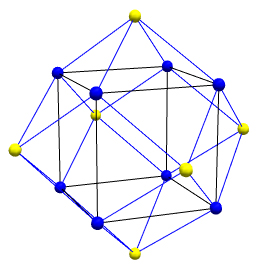
\includegraphics[scale=0.35]{../img/bunch.jpg}
    \caption{Linking between cell and transition nodes.}
    \label{FIG_BUNCH}
\end{figure}

\alglanguage{pseudocode}
\begin{algorithm}[h]
    \caption{Step 4 of 7}
    \small{
    \begin{algorithmic}[1]
        \algrestore{refinement}
        \For{\textbf{each} cell node}
            \State updates each current cell's direction pointer
        \EndFor
        \State
        \For{\textbf{each} transition node}
            \State updates each current node's quadruple connector
        \EndFor
        \algstore{refinement}
    \end{algorithmic}
    }
    \label{STEP_4_REFINEMENT}
\end{algorithm}

The first loop of Algorithm \ref{STEP_4_REFINEMENT} configures the
directional pointers of each cell node in the bunch. For instance,
pointer \textit{north} of front northeast cell is pointed to the
north transition node, while pointer \textit{south} is pointed to
the front southeast cell node. At the end of the loop, all
directional pointers of all cell nodes will be appropriately
configured.

The second loop configures the quadruple connectors of the
transition nodes. A scheme is defined to determine to which cell
each quadruple connector must point. This must be done in a very
precise way, as this choice will interfere in the simplification
procedure. Figure \ref{SCHEME_4CONNECTORS} shows the adopted scheme.

\begin{figure}[!ht]
    \centering
    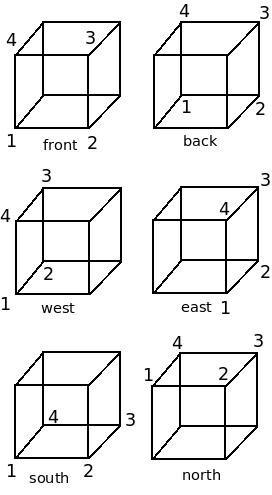
\includegraphics[scale=0.5]{../img/order_4connectors.jpg}
    \caption{Configuration scheme for quadruple connectors of the transition nodes.}
    \label{SCHEME_4CONNECTORS}
\end{figure}

For instance, as seen in the second cube in the second column of
Figure \ref{SCHEME_4CONNECTORS}, quadruple connectors 1, 2, 3 and 4
of transition node (\textit{east}) are respectively pointed to node
cells front southeast, back southeast, back northeast and front
northeast.


\subsubsection*{Step 5. Linking of the graph to the new bunch}
In step 3, after being created, the transition nodes of the new
bunch were pointed to the neighboring cells of the just refined
\textit{cellNode} thereby linking it to the graph of the mesh.
Reciprocally, the graph itself must be connected to the new bunch,
since all links in the graph are bidirectional; at this point in the
algorithm the neighboring nodes of the refined cell still point to
\textit{cellNode}, which no longer exists. This update is done by
Algorithm \ref{STEP_5_REFINEMENT}, where the neighboring nodes to
the refined cell are linked to the six transition nodes of the
bunch.

\alglanguage{pseudocode}
\begin{algorithm}[!hb]
    \caption{Step 5 of 7}
    \small{
    \begin{algorithmic}[1]
        \algrestore{refinement}
        \State $char$ $direction$
        \State $CellNode$  $neighborCN$
        \State $TransitionNode$  $neighborTN$
        \State $TransitionNode$ $transitionNode[6]$
        \State $transitionNode[0] \gets northTN$
        \State $transitionNode[1] \gets southTN$
        \State $transitionNode[2] \gets eastTN$
        \State $transitionNode[3] \gets westTN$
        \State $transitionNode[4] \gets frontTN$
        \State $transitionNode[5] \gets backTN$
        \State
        \For{i $\gets$ 0 \textbf{to} 5}
            \If{$transitionNode[i]\cdot singleConnector$ is a cell node}
                \State $neighborCN \gets transitionNode[i].singleConnector$
                \State $direction \gets transitionNode[i].direction$
                \State $neighborCN.oppositeDirection(direction) \gets transitionNode[i]$

            \Else \Comment{In this case the neighboring cell is a transition node}
                \State $neighborTN \gets transitionNode[i].singleConnector$
                \If{$neighborTN.singleConnector == cellNode$}
                    \State $neighborTN.singleConnector \gets transitionNode[i]$
                    \State
                \ElsIf{$neighborTN.quadrupleConnector1 == cellNode$}
                    \State $neighborTN.quadrupleConnector1 \gets transitionNode[i]$
                    \State
                \ElsIf{$neighborTN.quadrupleConnector2 == cellNode$}
                    \State $neighborTN.quadrupleConnector2 \gets transitionNode[i]$
                    \State
                \ElsIf{$neighborTN.quadrupleConnector3 == cellNode$}
                    \State $neighborTN.quadrupleConnector3 \gets transitionNode[i]$
                    \State
                \ElsIf{$neighborTN.quadrupleConnector4 == cellNode$}
                    \State $neighborTN.quadrupleConnector4 \gets transitionNode[i]$

                \Else
                    \State $print('Error')$
                \EndIf
            \EndIf
        \EndFor
        \algstore{refinement}
    \end{algorithmic}
    }
    \label{STEP_5_REFINEMENT}
\end{algorithm}

The neighboring nodes of the refined cell \textit{cellNode} can be
either cell nodes or transition nodes. When the neighbor node is a
cell node, the directional pointer of that node must be pointed to
the transition node whose direction is opposite to that of the
transition node. For example, assume that the north transition node
has a cell node as a neighbor, that is, its single connector points
to a cell node. This neighboring cell node must have its directional
pointer \textit{south} pointed to the north transition node. In
Algorithm \ref{STEP_5_REFINEMENT}, this task is executed in line 66,
where method \textit{oppositeDirection()} returns the directional
pointer whose direction is opposite to that received as a parameter.

In case the neighboring node of the transition node of the bunch is
also a transition node, then an analysis of its single connector and
all its quadruple connectors must be done in order to determine
which one points to \textit{cellNode}, which is the one who must be
updated and pointed to the transition node of the bunch. This
analysis and update are done by the piece of code between lines 67
and 86.

\subsubsection*{Step 6. Ordering of the cell nodes of the graph using the modified Hilbert curve}
The modified Hilbert curve is a space filling curve which is capable
of passing through all the points of a three-dimensional mesh
irrespective of how irregular this mesh might be. Its implementation
is done by means of a double chain list where each cell node
possesses two additional pointers: \textit{next} and
\textit{previous}. Any cell of the mesh can be reached traversing
the chain list defined by the Hilbert curve to the point it
occupies.

When a cell is refined, the 8 new cells of the bunch must be ordered
and inserted in the Hilbert curve, in order to be accessible later.
They are ordered in a small list, according to the relative position
of the refined cell in the Hilbert curve of the graph (before
refinement), which is later inserted in the main list. This
preordering in a sublist guarantees that the cells of the same bunch
will always be near each other in the ordering of the curve, causing
only a local modification in the curve. Therefore, inserting the new
cells in the main curve consists only in inserting an already
ordered sublist in the position of the cell just refined. The manner
in which this is done is detailed in Section
\ref{SEC_HILBERT_CURVE}. However, the implementation is done at this
step of the refinement, where the references for the pointers
\textit{next} and \textit{previous} of each cell of the bunch are
defined. Algorithm \ref{STEP_6_REFINEMENT} shows how this is
executed.

\alglanguage{pseudocode}
\begin{algorithm}[!ht]
    \caption{Step 6 of 7}
    \small{
    \begin{algorithmic}[1]
        \algrestore{refinement}
        \For{\textbf{each} cell node}
            \State sets current cell's next pointer according to modified Hilbert curve algorithm
            \State sets current cell's previous pointer according to modified Hilbert curve algorithm
        \EndFor
        \algstore{refinement}
    \end{algorithmic}
    }
    \label{STEP_6_REFINEMENT}
\end{algorithm}


\subsubsection*{Step 7. Removal of unnecessary transition nodes of the graph}
The function of the transition nodes in the ALG data structure is to
enable the communication between nodes of different levels of
refinement. In the refinement process, transition nodes are created
to connect the cells of the new bunch with the neighboring cells of
the refined cell. However, the neighborhood of the refined cell may
contain cells which have the same level of refinement of the cells
of the new bunch. In this situation a transition node is
dispensable, since the cells can be directly linked.

For instance, in Figure \ref{FIG_BEFORE_SIMPLIFY}, we have two
neighboring bunches whose cell nodes possess the same refinement
levels and which are connected by means of two transition nodes.
However, they can be directly connected as shown in Figure
\ref{FIG_AFTER_SIMPLIFY}.

%WITHOUT SIMPLIFICATION
\begin{figure}[!ht]
    \centering
    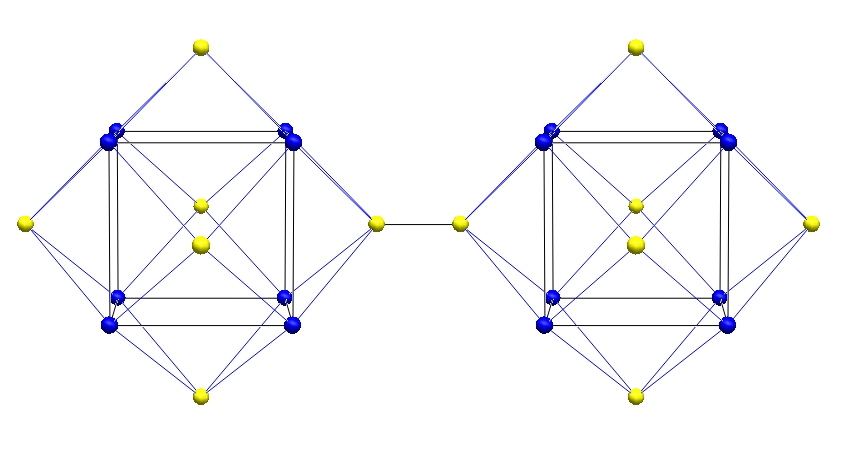
\includegraphics[scale=0.20,angle=0]{../img/graphNotSimplified.jpg}
    \caption{Graph before simplification showing two unnecessary transition nodes.}
    \label{FIG_BEFORE_SIMPLIFY}
\end{figure}


%WITH SIMPLIFICATION
\begin{figure}[!ht]
    \centering
    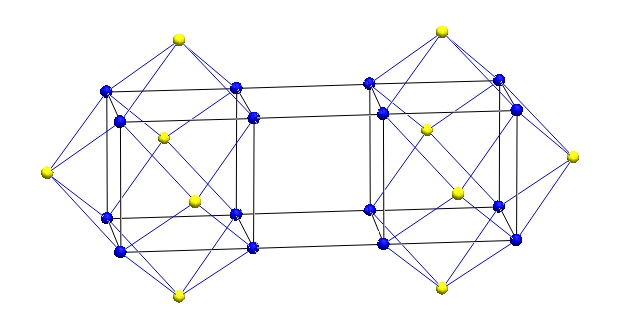
\includegraphics[scale=0.3,angle=0]{../img/graphSimplified.jpg}
    \caption{Simplified graph with transition nodes eliminated and cell nodes directly linked.}
    \label{FIG_AFTER_SIMPLIFY}
\end{figure}

In order to eliminate the storage problem associated with keeping
unnecessary transition nodes, the last step in the refinement
process contains a \textit{simplification} procedure that deletes
needless transition nodes in the new bunch and its immediate
neighborhood, as well as makes the direct link between nodes with
the same refinement level. This procedure is detailed in the next
subsection.

\alglanguage{pseudocode}
\begin{algorithm}[!ht]
    \caption{Step 7 of 7}
    \small{
    \begin{algorithmic}[1]
        \algrestore{refinement}
        \For{i $\gets$ 0 \textbf{to} 5}
            \State $simplifyRef(transitionNode[i])$
        \EndFor
        \EndProcedure
    \end{algorithmic}
    }
    \label{STEP_7_REFINEMENT}
\end{algorithm}


\subsection{Simplification routine} \label{SUBSEC_SIMPLIFICATION_REF}

The simplification routine is executed by the code described in
Algorithm \ref{SIMPLIFICATION_REFINEMENT}. In order for a
simplification to occur, two conditions must be satisfied. The first
one is that the single connector of a transition node received as a
parameter in function \textit{simplifyRef()} must point to a
transition node. The second condition is that they must possess the
same refinement level. In Algorithm
\ref{SIMPLIFICATION_REFINEMENT} these conditions are verified
in lines 2 and 3.

\alglanguage{pseudocode}
\begin{algorithm}[!hb]
    \caption{Simplification - Refinement}
    \small{
    \begin{algorithmic}[1]
    \Procedure{simplifyRef}{transitionNode}
    \If{$transitionNode.singleConnector.type == transitionNode.type$}
        \If{$transitionNode.singleConnector.level == transitionNode.level$}
            \State
            \State $TransitionNode$ $neighborTN \gets transitionNode.singleConnector$
            \State $char$ $dir \gets neighTN.direction$
            \State $CellNode$ $quadCon[4]$ \Comment{Stores the node's quadruple connectors}
            \State $Cell$ $nQuadCon[4]$ \Comment{Stores the neighbor node's quadruple connectors}
            \State
            \State $quadCon[0] \gets transitionNode.quadrupleConnector1$
            \State $quadCon[1] \gets transitionNode.quadrupleConnector2$
            \State $quadCon[2] \gets transitionNode.quadrupleConnector3$
            \State $quadCon[3] \gets transitionNode.quadrupleConnector4$
            \State
            \State $nQuadCon[0] \gets neighborTN.quadrupleConnector1$
            \State $nQuadCon[1] \gets neighborTN.quadrupleConnector2$
            \State $nQuadCon[2] \gets neighborTN.quadrupleConnector3$
            \State $nQuadCon[3] \gets neighborTN.quadrupleConnector4$

            \State
            \For{$i \gets 0$ \textbf{to} $3$}
                \State $quadCon[i].oppositeDirection(dir) \gets nQuadCon[i]$
            \EndFor
            \State $dir \gets transitionNode.direction$
            \For{$i \gets 0$ \textbf{to} $3$}
                \If{$nQuadCon[i]$ is a cell node}
                    \State $nQuadCon[i].oppositeDirection(dir) \gets quadCon[i]$
                \Else

                    \If{$neighborTN == nQuadCon[i].singleConnector$}
                        \State $nQuadCon[i].singleConnector \gets quadCon[i]$
                    \ElsIf{$neighborTN == nQuadCon[i].quadrupleConnector1$}
                        \State $nQuadCon[i].quadrupleConnector1 \gets quadCon[i]$
                    \ElsIf{$neighborTN == nQuadCon[i].quadrupleConnector2$}
                        \State $nQuadCon[i].quadrupleConnector2 \gets quadCon[i]$
                    \ElsIf{$neighborTN == nQuadCon[i].quadrupleConnector3$}
                        \State $nQuadCon[i].quadrupleConnector3 \gets quadCon[i]$
                    \ElsIf{$neighborTN == nQuadCon[i].quadrupleConnector4$}
                        \State $nQuadCon[i].quadrupleConnector4 \gets quadCon[i]$
                    \Else
                        \State $print('Error')$
                    \EndIf
                \EndIf
            \EndFor
            \State
            \State \textbf{delete} $transitionNode$
            \State \textbf{delete} $neighborTN$
        \EndIf
    \EndIf
    \EndProcedure
    \end{algorithmic}
    }
    \label{SIMPLIFICATION_REFINEMENT}
\end{algorithm}

When both conditions are obeyed, the graph must be simplified.
Before removing the unnecessary transition nodes, the references of
their quadruple connectors must be stored, since they are the
references for the cell nodes which will be directly linked.

In Algorithm \ref{SIMPLIFICATION_REFINEMENT}, vector \textit{quadCon}
stores references for the quadruple connectors of the transition
node (\textit{transitionNode}) received as a parameter; vector
\textit{nQuadCon} stores references for the quadruple connectors of
the neighbor transition node (\textit{neighborTN}) which is pointed
to by the single connector of \textit{transitionNode}.

Thereafter, the cells of the bunch which are referenced by the
quadruple connectors of \textit{transitionNode} are pointed to those
referenced by the quadruple connectors of \textit{neighborTN}. This
is done by the loop between lines 20 and 22. The directional pointer
of each one of these nodes that must be reconfigured is the one
whose direction is opposite of that of \textit{neighborTN}. For
instance, assume in Figure \ref{FIG_BEFORE_SIMPLIFY} that the west
transition node of the right-hand bunch is passed as a parameter to
the simplification routine. Then the nodes which are referenced by
its quadruple connectors will point their \textit{west} directional
pointers to the nodes referenced by the quadruples connectors of the
east transition node of the left-hand side bunch. Here the scheme
depicted in Figure \ref{SCHEME_4CONNECTORS} guarantees that the
connections are correctly done.

Next the cells of the bunch which are referenced by the quadruple
connectors of \textit{neighborTN} are pointed to those referenced by
the quadruple connectors of \textit{transitionNode}. These nodes can
be either cell nodes or transition nodes. If they are cell nodes,
the directional pointer that must be reconfigured is that with
direction opposite to the one of \textit{transitionNode}. This is
done in line 26 of Algorithm \ref{SIMPLIFICATION_REFINEMENT}.
If they are transition nodes, one must first find out which type of
connector of these nodes points to \textit{neighborTN}. This is done
by the piece of code between lines 27 and 45.

After all neighbor nodes with the same refinement levels are
connected, the transition nodes \textit{transitionNode} and
\textit{neighborTN} are removed from the graph.
